\documentclass[a4paper,12pt]{article}
\usepackage{amsmath}
\usepackage{graphicx}
\begin{document}
\newcommand{\del}{\nabla}
\textbf{ } \\
\textbf{ANKIT MAHATO} \\
\textbf{Y9227099} \\
\\
\\
\textbf{Problem 1} \\
\\
The Hilbert matrix, known to be severely ill‐conditioned, is defined as \\
\[
H_n =
  \begin{bmatrix}
    1 & 1/2 & 1/3 & .. & 1/N\\
    1/2 & 1/3 & .. & .. & 1/(N+1)\\
    1/3 & . & .. & .. & .\\
    . & . & . & .. & .\\
    1/N & .. & .. & .. & 1/(2N-1)\\
  \end{bmatrix}
\]
\\
Condition Number($H_n$) = $|||H_n|||$ $|||{H_n}^{-1}|||$ \\
The elements of $H_n$ is given by\\
\[ H_{n_{ij}} = \frac{1}{(i + j -1)}  \]
The elements of $H^{-1}_n$ is given by\\
\[ H^{-1}_{n_{ij}} = \frac{(-1)^{i+j} c_i c_j}{(i + j -1)}  \]
where\\
\[ c_i = \frac{(n+i-1)!}{(n-i)!((i-1)!)^2}  \]
\\
(i)\\
We calculate the 1-norm of the hilbert matrix and its inverse using:\\
\[ ||A||_1 = max(\sum_{j=1}^n A_{1j}, \sum_{j=1}^n A_{2j}, .., \sum_{j=1}^n A_{nj}) \] 
\\
\newpage
\textbf{ } \\
After calculating using MATLAB code.\\
\\
\textbf{Table}\\
\\
\begin{tabular}{ l r r r }
 N & $||H_n||$ & $||H^{-1}_n||$ & Condition Number(K)\\
 1 & 1.000 & 1 & 1 \\
 2 & 1.500 & 18 & 27 \\
 3 & 1.833 & 408 & 748 \\
 4 & 2.083 & 13620 & 28375 \\
 5 & 2.283 & 413280 & 943656 \\
 6 & 2.450 & 11865420 & 29070279 \\
\end{tabular}
\\
\\
After N=5 CN exceeds $10^6$.\\
CN as a function of N upto N=5 is given by the plot below\\
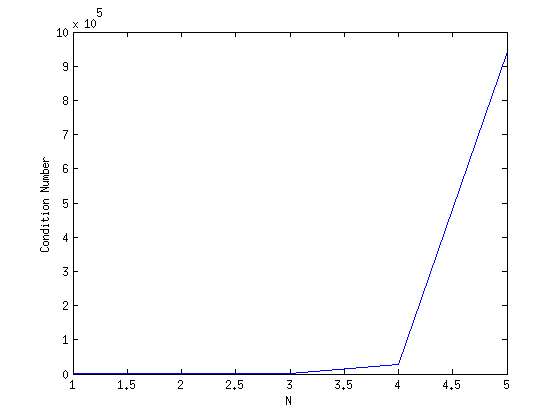
\includegraphics [keepaspectratio=true] {1norm.png}
\newpage
\textbf{ } \\
(ii)\\
We calculate the 2-norm of the hilbert matrix and its inverse using:\\
\[ ||A||_2 = \sqrt{\lambda_{max}(A\times A)} \] 
where $\lambda_max$ is the maximum among the eigen values.\\
After calculating using MATLAB code.\\
\\
\textbf{Table}\\
\\
\begin{tabular}{ l r r r }
 N & $||H_n||$ & $||H^{-1}_n||$ & Condition Number(K)\\
 1 & 1.000 & 1 & 1 \\
 2 & 1.267 & 15.211 & 19.281 \\
 3 & 1.408 & 372.115 & 524.057 \\
 4 & 1.500 & 10341.015 & 15513.739 \\
 5 & 1.567 & 304142.842 & 476607.250 \\
 6 & 1.619 & 9235320.244 & 14951058.640 \\
\end{tabular}
\\
After N=5 CN exceeds $10^6$.\\
\newpage
\textbf{ } \\
CN as a function of N upto N=5 is given by the plot below\\
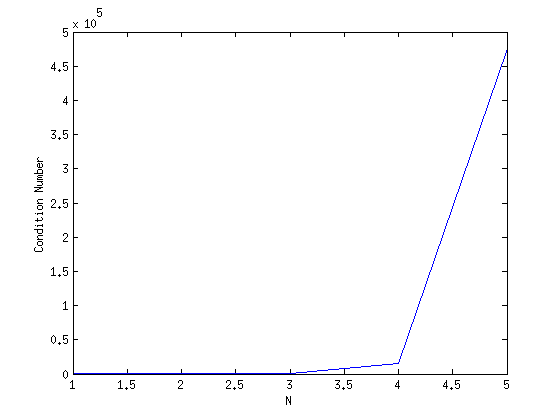
\includegraphics [keepaspectratio=true] {2norm.png}
\\
\\
\textbf{Problem 2} \\
\\
\begin{tabular}{ r r }
 x & y\\
    0.1 & 10.57 \\
    0.2 & 19.03 \\
    0.5 & 36.61 \\ 
    0.7 & 44.43 \\
    1.0 & 52.92 \\
    2.0 & 68.16 \\
    5.0 & 82.65 \\
    7.0 & 86.30 \\
   10.0 & 89.46 \\
\end{tabular}
\newpage
\textbf{ } \\
The saturation curve is given by\\
\[ y = \frac{\alpha x}{\beta + x}  \]
\[ \frac{1}{y} = \frac{\beta}{\alpha} \frac {1}{x} + \frac{1}{\alpha}  \]
Now we can perform linear regression and determine the constants $\beta$ and $\alpha$ using the matlab code\\
Their values are\\
\[ \alpha =  95.8729 \]
\[ \beta =  0.8073 \]
The correlation coefficient is equal to 1 which suggests perfect positive fit as shown by the plot of 1/y vs 1/x below:\\
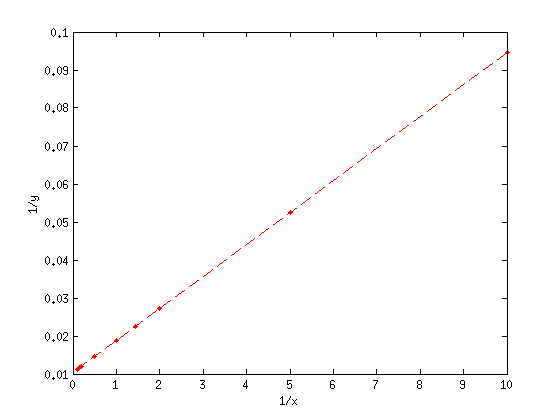
\includegraphics [keepaspectratio=true] {prob21.png}
\\
The y vs x curve generated using the new model is shown below\\
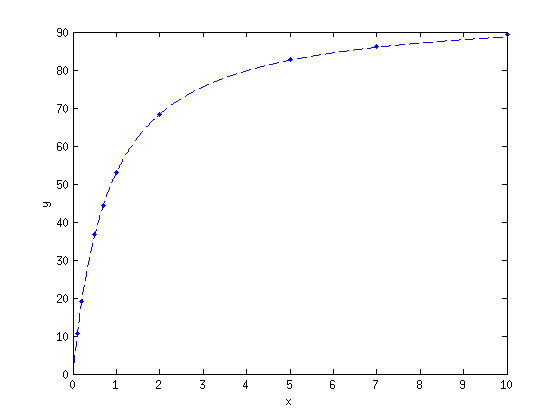
\includegraphics [keepaspectratio=true] {prob22.png}
\end{document}